\chapter{Az SVG és eszközkészlete}
\label{ch:svg}

A fejezet első fele az SVG azon elemeit mutatja be, amelyekkel egy szerkesztőnek dolgoznia kell, a második fele pedig öt elterjedt SVG-szerkesztőt hasonlít össze. Az összehasonlítás szempontjai adják \aref{ch:requirements}. fejezetben megfogalmazott követelmények vázát.

\section{Az SVG grafikus elemei}
\label{sec:svg_graphical_elements}

A Scalable Vector Graphics (SVG) XML-alapú nyelv kétdimenziós vektorgrafikák leírására. A dokumentum hierarchikus felépítésű, minden grafikus objektum egy közös gyökérelembe, az \lstinline[language=XML]|<svg>| kezdő és záró címkéje közé kerül, ahogyan az alábbi kódrészlet mutatja.

\begin{lstlisting}[language=XML]
    <svg xmlns="http://www.w3.org/2000/svg"
        width="100" height="100">
        <!-- SVG-elemek -->
    </svg>
\end{lstlisting}

Az SVG koordináta-rendszerének origója a bal felső sarokban van, és a matematikai ábrázolással ellentétben az y tengely lefelé mutat.

\paragraph{A \texttt{viewBox} attribútum}
Az \lstinline[language=XML]|<svg>| elem opcionális \lstinline[language=XML]|viewBox| attribútuma egy saját koordináta-rendszert határoz meg a tartalom számára, amelyet a böngésző a \texttt{width} és \texttt{height} attribútumokban megadott méretre skáláz. Az értéke négy szám: \texttt{min-x}, \texttt{min-y}, \texttt{width} és \texttt{height}. Ha hiányzik, egy koordinátaegység egy CSS-képpontnak felel meg. \Aref{fig:example_viewbox}. ábrán a \texttt{viewBox} egy 0-tól 100-ig terjedő koordináta-rendszert ad meg, a tartalom pedig kitölti a 400$\times$400 képpontos területet.

\begin{figure}[H]
    \centering
    \begin{adjustbox}{valign=m, max width=0.7\textwidth}
        \begin{lstlisting}[language=XML]
        <svg xmlns="http://www.w3.org/2000/svg"
            width="400" height="400" viewBox="0 0 100 100">
            <circle cx="50" cy="50" r="40"
                fill="lightgray" stroke="black" stroke-width="2"/>
        </svg>
        \end{lstlisting}
    \end{adjustbox}
    \hfill
    \begin{adjustbox}{valign=m, max width=0.2\textwidth}
        \includesvg{images/concept/viewbox.svg}
    \end{adjustbox}
    \caption{A viewBox attribútum hatása a koordináta-rendszerre}
    \label{fig:example_viewbox}
\end{figure}

A szakasz először a megjelenést befolyásoló attribútumokat ismerteti (\ref{sub:vis_attrs}.~alszakasz), majd az alapalakzatokat (\ref{sub:basic_shapes}.~alszakasz), az útvonalakat (\ref{sub:paths}.~alszakasz), a szöveget és a képeket (\ref{sub:other_elements}.~alszakasz), végül a csoportosítást, az újrafelhasználható definíciókat és a színátmeneteket (\ref{sub:group_defs}.~alszakasz). Az elemek használatát kódrészletek és a hozzájuk tartozó ábrák mutatják be.

\subsection{Megjelenési attribútumok}
\label{sub:vis_attrs}

Az elemek kinézetét a geometriájuk mellett a megjelenési attribútumok határozzák meg~\cite{mdn-svg-attributes,w3c-svg-painting}. Ezek CSS-tulajdonságként is megadhatók, így szerepelhetnek attribútumként az elemen, a \texttt{style} attribútumban vagy egy stíluslapon.

\subsubsection{Körvonal}

A körvonal az alakzat határvonala. Az SVG a színe és vastagsága mellett a vonal végződését, a sarkok alakját és a szaggatást is leírja.

\begin{description}
\item[\texttt{stroke}] A körvonal színe. Értéke színkód, színnév vagy hivatkozás egy színátmenetre. Alapértéke \texttt{none}, vagyis a körvonal nem látszik.
\item[\texttt{stroke-width}] A vonalvastagság az aktuális koordináta-rendszer egységében. Alapértéke 1.
\item[\texttt{stroke-opacity}] A körvonal átlátszatlansága 0 és 1 között, ahol 0 a teljesen átlátszó. A kitöltés átlátszatlanságát nem befolyásolja.
\item[\texttt{stroke-linecap}] A nyitott útvonalak végpontjainak alakja, \aref{fig:example_stroke-linecap}. ábra szerint.
\begin{description}
    \item[\texttt{butt}] A vonal pontosan a végpontban ér véget. Ez az alapérték.
    \item[\texttt{round}] A vonal végét egy félkör zárja le, amelynek sugara a vonalvastagság fele.
    \item[\texttt{square}] A vonal négyzetes véggel a vonalvastagság felével túlnyúlik a végponton.
\end{description}
\end{description}

\begin{figure}[H]
    \centering
    \includesvg[width=0.2\textwidth]{images/concept/stroke-linecap.svg}
    \caption{A stroke-linecap attribútum három értéke}
    \label{fig:example_stroke-linecap}
\end{figure}

\begin{description}
\item[\texttt{stroke-linejoin}] Két szakasz találkozásánál a sarok alakja, \aref{fig:example_stroke-linejoin}. ábra szerint.
\begin{description}
    \item[\texttt{miter}] Hegyes sarok, a külső élek a metszéspontjukig hosszabbodnak meg. Ez az alapérték.
    \item[\texttt{round}] Lekerekített sarok.
    \item[\texttt{bevel}] Levágott sarok, a két szakasz külső sarokpontjait egy egyenes köti össze.
\end{description}
Az SVG 2 két további értéket vezetett be, a \texttt{miter-clip} és az \texttt{arcs} értéket, ezeket azonban a böngészők még nem támogatják széles körben~\cite{mdn-linejoin}.
\end{description}

\begin{figure}[H]
    \centering
    \includesvg[width=0.2\textwidth]{images/concept/stroke-linejoin.svg}
    \caption{A stroke-linejoin attribútum három értéke}
    \label{fig:example_stroke-linejoin}
\end{figure}

\begin{description}
\item[\texttt{stroke-dasharray}] A szaggatott vonal mintáját adja meg vesszővel vagy szóközzel elválasztott számokkal, amelyek felváltva a vonalszakaszok és a hézagok hosszát adják meg. A hosszak az aktuális koordináta-rendszer egységében értendők, a minta tehát nem igazodik a vonalvastagsághoz.
\item[\texttt{stroke-dashoffset}] A szaggatási minta kezdőpontjának eltolása az útvonal elejéhez képest. Vele a minta megváltoztatása nélkül csúsztatható el a szaggatás.
\end{description}

\subsubsection{Kitöltés}

A kitöltés az alakzat belső területét színezi. Nyitott útvonalnál az a terület számít belsőnek, amely a végpontok egyenes összekötésével jönne létre.

\begin{description}
\item[\texttt{fill}] A belső terület színe. A körvonalhoz hasonlóan lehet szín, színátmenet vagy minta. Alapértéke fekete, a \texttt{none} érték mellett a belső terület üres marad.
\item[\texttt{fill-opacity}] A kitöltés átlátszatlansága 0 és 1 között. A körvonal átlátszatlanságát nem befolyásolja.
\item[\texttt{fill-rule}] Önmagát metsző vagy lyukas útvonalaknál azt dönti el, mely területek számítanak belsőnek. A vizsgált pontból tetszőleges irányban egy félegyenest húzunk, és az útvonallal alkotott metszéspontjait vizsgáljuk.
\begin{description}
    \item[\texttt{nonzero}] Az alapszabály. Ahol az útvonal az egyik irányban keresztezi a félegyenest, ott eggyel nő, ahol a másikban, ott eggyel csökken egy számláló. A pont akkor belső, ha a számláló végül nem nulla.
    \item[\texttt{evenodd}] A pont akkor belső, ha a metszéspontok száma páratlan. Ezzel a szabállyal egy külső és egy belső kontúrból egyszerűen készíthető lyukas alakzat.
\end{description}
\end{description}

\begin{figure}[H]
    \centering
    \includesvg[width=0.2\textwidth]{images/concept/fill-rule.svg}
    \caption{A fill-rule attribútum két értéke}
    \label{fig:example_fill-rule}
\end{figure}

\subsubsection{Átlátszóság}

Az \texttt{opacity} attribútum az egész elem átlátszatlanságát adja meg 0 és 1 között. A \texttt{fill-opacity} és a \texttt{stroke-opacity} attribútumtól abban különbözik, hogy csoportra alkalmazva a csoport tartalmát egy egységként halványítja el. Az egymást fedő tagok ezért nem látszanak át egymáson, csak a csoport egésze lesz áttetsző.

\subsubsection{Transzformációk}

A \texttt{transform} attribútum az elem koordináta-rendszerét alakítja át~\cite{mdn-transform}. Az elemet a \texttt{translate(x, y)} függvény eltolja, a \texttt{rotate(a, x, y)} az $(x, y)$ pont körül $a$ fokkal elforgatja, a \texttt{scale(x, y)} pedig a két tengely mentén méretezi. Egyetlen paraméterrel, \texttt{scale(s)} alakban mindkét irányban ugyanakkora a méretezés. A \texttt{skewX} és \texttt{skewY} függvény nyírást ír le, a \texttt{matrix} pedig hat számmal tetszőleges affin transzformációt, vagyis az eltolás, a forgatás, a méretezés és a nyírás bármely kombinációját. Több transzformáció egymás után is felsorolható.

\subsubsection{Szűrők, vágás, maszkolás és animáció}

Az SVG ennél több megjelenítési lehetőséget is kínál, ezek azonban túlmutatnak az elkészült szerkesztőn. A \texttt{filter} elem szűrőprimitívekből épít fel összetett hatásokat, például elmosást vagy árnyékot~\cite{mdn-filter}. A \texttt{clipPath} elem vágóútvonalat határoz meg, amelyen kívül az elem nem látszik~\cite{mdn-clippath}, a \texttt{mask} elem pedig a maszk világosságával vagy átlátszatlanságával fokozatosan teszi láthatóvá az elemet~\cite{mdn-mask}. Az attribútumok időbeli változása a SMIL nyelvből átvett \texttt{animate}, \texttt{animateTransform} és \texttt{animateMotion} elemekkel írható le~\cite{mdn-smil}. Ezek kezelése a továbbfejlesztési lehetőségek közé tartozik, a szerkesztő importálója figyelmeztetést ad, ha egy fájl ilyen elemeket tartalmaz.

\subsection{Alapalakzatok}
\label{sub:basic_shapes}

Az SVG hat alapalakzatot ismer~\cite{mdn-svg-elements}, amelyek egy-egy egyszerű geometriai formát néhány attribútummal írnak le. \Aref{tab:basic-shapes}. táblázat az alakzatokat meghatározó attribútumokat foglalja össze, \aref{fig:basic-shapes}. ábra pedig mind a hatot bemutatja.

\begin{table}[!ht]
\caption{Az SVG alapalakzatai és meghatározó attribútumaik}
\label{tab:basic-shapes}
\centering
\footnotesize
\renewcommand{\arraystretch}{1.2}
\begin{tabular}{|l|l|>{\raggedright\arraybackslash}p{0.5\textwidth}|}
\hline
\textbf{Alakzat} & \textbf{Elem} & \textbf{Attribútumok} \\ \hline
vonal & \texttt{<line>} & \texttt{x1}, \texttt{y1} és \texttt{x2}, \texttt{y2}: a két végpont \\ \hline
téglalap & \texttt{<rect>} & \texttt{x}, \texttt{y}: a bal felső sarok; \texttt{width}, \texttt{height}: a méret; \texttt{rx}, \texttt{ry}: a sarkok lekerekítésének sugara \\ \hline
kör & \texttt{<circle>} & \texttt{cx}, \texttt{cy}: a középpont; \texttt{r}: a sugár \\ \hline
ellipszis & \texttt{<ellipse>} & \texttt{cx}, \texttt{cy}: a középpont; \texttt{rx}, \texttt{ry}: a vízszintes és a függőleges sugár \\ \hline
sokszög & \texttt{<polygon>} & \texttt{points}: a csúcsok \texttt{x,y} párjai bejárási sorrendben \\ \hline
töröttvonal & \texttt{<polyline>} & \texttt{points}: a töréspontok, mint a sokszögnél \\ \hline
\end{tabular}
\end{table}

A sokszög utolsó csúcsát az elem automatikusan összeköti az elsővel, ezért a kezdőpontot nem kell megismételni. A töröttvonal ugyanígy írható le, de nyitva marad. A kitöltés ennek ellenére a zárt területre vonatkozik, ahogyan \aref{fig:basic-shapes}. ábra jobb alsó részén a szürke terület mutatja.

\begin{figure}[!ht]
    \centering
    \begin{adjustbox}{valign=m, max width=0.52\textwidth}
        \begin{lstlisting}[language=XML]
<line x1="10" y1="10" x2="90" y2="90"
  stroke="blue" stroke-width="2"/>
<rect x="20" y="30" width="60" height="40"
  rx="10" ry="10"/>
<circle cx="50" cy="50" r="30"/>
<ellipse cx="50" cy="50" rx="40" ry="25"/>
<polygon points="50,10 90,90 10,90"/>
<polyline
  points="10 90, 30 10, 50 70, 70 30, 90 90"/>
        \end{lstlisting}
    \end{adjustbox}
    \hfill
    \begin{adjustbox}{valign=m, max width=0.44\textwidth}
        \includesvg{images/concept/basic-shapes.svg}
    \end{adjustbox}
    \caption{A hat alapalakzat. Mindegyik a saját $100\times100$ egységes cellájában áll, a kitöltés világosszürke, a körvonal fekete.}
    \label{fig:basic-shapes}
\end{figure}

\subsection{Útvonalak}
\label{sub:paths}

A \lstinline[language=XML]|<path>| elem a legáltalánosabb alakzat, minden más alakzat leírható vele. Az alakját a \texttt{d} attribútum parancsai adják meg. Minden parancs egy betűből és a paramétereiből áll. A nagybetűs parancsok paraméterei abszolút koordináták, a kisbetűseké az aktuális ponthoz képesti eltolások. A paraméterek többnyire koordinátapárok, az ív azonban szöget és két jelzőbitet is kap.

\subsubsection{Egyenes szakaszok}

Az egyenes szakaszokat az alábbi parancsok írják le.

\begin{itemize}
\item \texttt{M}, \texttt{m}: áthelyezi az aktuális pontot rajzolás nélkül, mintha a tollat felemelnénk
\item \texttt{L}, \texttt{l}: egyenes szakasz az aktuális ponttól a megadott pontig
\item \texttt{H}, \texttt{h}: vízszintes szakasz
\item \texttt{V}, \texttt{v}: függőleges szakasz
\item \texttt{Z}, \texttt{z}: egyenes szakasszal visszazárja az útvonalat a kezdőpontjába
\end{itemize}

\Aref{fig:example_path_line}. ábra útvonala egy négyszöget rajzol, amely a $(10, 20)$ pontból indul, és a \texttt{Z} paranccsal zárul.

\begin{figure}[H]
    \centering
    \begin{adjustbox}{valign=m, max width=0.8\textwidth}
        \begin{lstlisting}[language=XML]
    <path d="M 10,20 L 80,10 L 50,90 L 20,80 Z"
        fill="lightgray" stroke="black"
        stroke-width="2"/>
        \end{lstlisting}
    \end{adjustbox}
    \hfill
    \begin{adjustbox}{valign=m, max width=0.2\textwidth}
        \includesvg{images/concept/path-line.svg}
    \end{adjustbox}
    \caption{Egyenes szakaszokból álló zárt útvonal kódja és megjelenése}
    \label{fig:example_path_line}
\end{figure}


\subsubsection{Bézier-görbék}

A Bézier-görbék alakját kontrollpontok határozzák meg~\cite{mdn-bezier,bezier-primer,farin2002}. A görbe a két végpontján áthalad, a kontrollpontokon általában nem, azok csak a görbe irányát és ívét szabják meg. A grafikus szerkesztők a kontrollpontokat fogantyúként jelenítik meg, amelyek a végpontokhoz kötött szakaszok végén mozgathatók. Az SVG a másod- és a harmadfokú Bézier-görbét ismeri.

\paragraph{Másodfokú Bézier-görbe.} Egyetlen kontrollpontja van, amely a kezdő- és a végpont érintőjének irányát egyszerre határozza meg. A \texttt{Q}, \texttt{q} paranccsal rajzolható.

\begin{figure}[H]
    \centering
    \begin{adjustbox}{valign=m, max width=0.8\textwidth}
        \begin{lstlisting}[language=XML]
    <path d="M 90,90 Q 30,80 10,10"
        fill="none" stroke="blue"
        stroke-width="3"/>
        \end{lstlisting}
    \end{adjustbox}
    \hfill
    \begin{adjustbox}{valign=m, max width=0.2\textwidth}
        \includesvg{images/concept/path-quad-bezier.svg}
    \end{adjustbox}
    \caption{Másodfokú Bézier-görbe a kontrollpontjával}
    \label{fig:example_path_quad_bezier}
\end{figure}

\paragraph{Harmadfokú Bézier-görbe.} Két kontrollpontja közül az első a görbe kezdeténél, a második a végénél határozza meg az irányt. A \texttt{C}, \texttt{c} paranccsal rajzolható.

\begin{figure}[H]
    \centering
    \begin{adjustbox}{valign=m, max width=0.8\textwidth}
        \begin{lstlisting}[language=XML]
    <path d="M 90,90 C 50,83 23,57 10,10"
        fill="none" stroke="blue"
        stroke-width="3"/>
        \end{lstlisting}
    \end{adjustbox}
    \hfill
    \begin{adjustbox}{valign=m, max width=0.2\textwidth}
        \includesvg{images/concept/path-cubic-bezier.svg}
    \end{adjustbox}
    \caption{Harmadfokú Bézier-görbe a két kontrollpontjával}
    \label{fig:example_path_cubic_bezier}
\end{figure}

\subsubsection{Ív}
\label{sub:arc}

Az \texttt{A}, \texttt{a} parancs egy ellipszis ívét rajzolja az aktuális ponttól a megadott végpontig. Ez a legtöbb paraméterrel rendelkező útvonalparancs:

\begin{itemize}
\item \texttt{rx}, \texttt{ry}: az ellipszis vízszintes és függőleges sugara
\item \texttt{x-axis-rotation}: az ellipszis x tengelyének elforgatási szöge
\item \texttt{large-arc-flag}: a kezdő- és végponton átmenő lehetséges ívek közül a legfeljebb 180 fokosat (0) vagy a nagyobbat (1) választja
\item \texttt{sweep-flag}: az ív haladási iránya, 1 esetén pozitív, 0 esetén negatív szögirányban; mivel az y tengely lefelé mutat, a pozitív irány a képernyőn az óramutató járásával egyezik meg
\item \texttt{x}, \texttt{y}: az ív végpontja
\end{itemize}

A következő négy ábra a paraméterek hatását mutatja. A kód pirossal kiemelt része az előző ábrához képest változott.

\begin{figure}[H]
    \centering
    \begin{adjustbox}{valign=m, max width=0.8\textwidth}
        \begin{lstlisting}[language=XML, escapeinside={!}{!}]
    <path d="M 25,50
        A !\textcolor{red}{29.5,50}! 0 0 0 75,50"
        fill="none" stroke="blue" stroke-width="3">
    </path>
        \end{lstlisting}
    \end{adjustbox}
    \hfill
    \begin{adjustbox}{valign=m, max width=0.2\textwidth}
        \includesvg{images/concept/path-arc-radi.svg}
    \end{adjustbox}
    \caption{Az rx és ry paraméter hatása. A kék ív egy képzeletbeli ellipszis része, a piros vonalak a sugarakat jelölik.}
    \label{fig:example_arc_radi}
\end{figure}

\begin{figure}[H]
    \centering
    \begin{adjustbox}{valign=m, max width=0.8\textwidth}
        \begin{lstlisting}[language=XML, escapeinside={!}{!}]
    <path d="M 25,50
        A 29.5,50 !\textcolor{red}{25}! 0 0 75,50"
        fill="none" stroke="blue" stroke-width="3">
    </path>
        \end{lstlisting}
    \end{adjustbox}
    \hfill
    \begin{adjustbox}{valign=m, max width=0.2\textwidth}
        \includesvg{images/concept/path-arc-rot.svg}
    \end{adjustbox}
    \caption{Az x-axis-rotation paraméter hatása}
    \label{fig:example_arc_rot}
\end{figure}

\begin{figure}[H]
    \centering
    \begin{adjustbox}{valign=m, max width=0.8\textwidth}
        \begin{lstlisting}[language=XML, escapeinside={!}{!}]
    <path d="M 25,50
        A 29.5,50 25 !\textcolor{red}{1}! 0 75,50"
        fill="none" stroke="blue" stroke-width="3">
    </path>
        \end{lstlisting}
    \end{adjustbox}
    \hfill
    \begin{adjustbox}{valign=m, max width=0.2\textwidth}
        \includesvg{images/concept/path-arc-large.svg}
    \end{adjustbox}
    \caption{A large-arc-flag paraméter hatása, a szaggatott vonal a másik érték szerinti ív}
    \label{fig:example_arc_large}
\end{figure}

\begin{figure}[H]
    \centering
    \begin{adjustbox}{valign=m, max width=0.8\textwidth}
        \begin{lstlisting}[language=XML, escapeinside={!}{!}]
    <path d="M 25,50
        A 29.5,50 25 0 !\textcolor{red}{1}! 75,50"
        fill="none" stroke="blue" stroke-width="3">
    </path>
        \end{lstlisting}
    \end{adjustbox}
    \hfill
    \begin{adjustbox}{valign=m, max width=0.2\textwidth}
        \includesvg{images/concept/path-arc-sweep.svg}
    \end{adjustbox}
    \caption{A sweep-flag paraméter hatása, a szaggatott vonal a másik érték szerinti ív}
    \label{fig:example_arc_sweep}
\end{figure}


\subsubsection{Összetett útvonalak}

Egy \lstinline[language=XML]|<path>| elemen belül az egyenes szakaszok, a Bézier-görbék és az ívek tetszőleges sorrendben követhetik egymást, így szabálytalan alakzatok is leírhatók egyetlen elemmel. \Aref{fig:example_freehand}. ábra egy másodfokú és egy harmadfokú görbét kapcsol össze.

\begin{figure}[H]
    \centering
    \begin{adjustbox}{valign=m, max width=0.8\textwidth}
        \begin{lstlisting}[language=XML]
    <path d="M10,50 Q50,120 40,20 C10,60 20,30 90,30"
        fill="none" stroke="blue" stroke-width="3"/>
        \end{lstlisting}
    \end{adjustbox}
    \hfill
    \begin{adjustbox}{valign=m, max width=0.2\textwidth}
        \includesvg{images/concept/path-freehand.svg}
    \end{adjustbox}
    \caption{Különböző parancsokból összeállított útvonal kódja és megjelenése}
    \label{fig:example_freehand}
\end{figure}


\subsection{Szöveg és kép}
\label{sub:other_elements}

Egy rajz a geometriai alakzatok mellett gyakran tartalmaz szöveget és raszteres képet is.

\subsubsection{Szöveg}

A szöveget a \lstinline[language=XML]|<text>| elem helyezi el. A szöveg karakterekként tárolódik, ezért kijelölhető, kereshető, és nagyításkor is éles marad.

\begin{itemize}
    \item \texttt{x}, \texttt{y}: az első karakter alapvonalának kezdőpontja
    \item \texttt{dx}, \texttt{dy}: eltolás az előző karakterhez képest
    \item \texttt{rotate}: az egyes karakterek elforgatása
    \item \texttt{fill}, \texttt{stroke}: a karakterek kitöltése és körvonala
\end{itemize}

A betűtípust a \texttt{font-family}, a méretet a \texttt{font-size} tulajdonság adja meg, a \lstinline[language=XML]|<tspan>| elem pedig a szöveg egy részének ad eltérő stílust vagy pozíciót. A \texttt{font-family} csak a betűtípus nevét rögzíti. Ha a fájlt megnyitó gépen nincs ilyen betűtípus, a böngésző egy másikat választ helyette, és a szöveg szélessége, tördelése és megjelenése megváltozik. Ez kétféleképpen kerülhető el. A betűtípus beágyazható a fájlba, vagy a szöveg útvonallá alakítható. Az utóbbi után a szöveg nem szerkeszthető tovább szövegként, viszont minden környezetben ugyanúgy jelenik meg.

\begin{figure}[H]
    \centering
    \begin{adjustbox}{valign=m, max width=0.8\textwidth}
        \begin{lstlisting}[language=XML]
        <text x="2" y="55" rotate="10" font-size="11"
          fill="gray" stroke="black" stroke-width="0.3">
          Szöveg <tspan fill="blue">kiemelés</tspan>
        </text>
        \end{lstlisting}
    \end{adjustbox}
    \hfill
    \begin{adjustbox}{valign=m, max width=0.17\textwidth}
        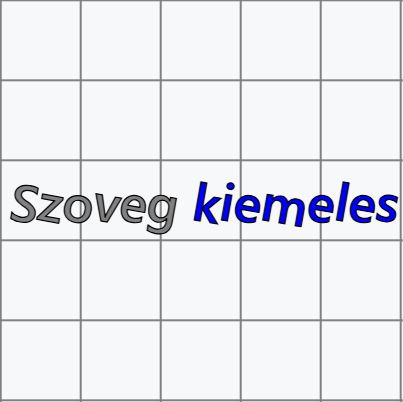
\includegraphics{images/concept/text.JPG}
    \end{adjustbox}
    \caption{Karakterenként elforgatott szöveg egy eltérő színű \texttt{<tspan>} résszel}
    \label{fig:example_text}
\end{figure}


\subsubsection{Raszteres kép}

Az \lstinline[language=XML]|<image>| elem raszteres képet, például PNG- vagy JPEG-fájlt helyez el a rajzban.

\begin{itemize}
    \item \texttt{x}, \texttt{y}: a kép bal felső sarka
    \item \texttt{width}, \texttt{height}: a kép megjelenített mérete
    \item \texttt{href}: a kép címe
\end{itemize}

A \texttt{href} hivatkozhat külső fájlra, de tartalmazhatja magát a képet is base64 kódolású \texttt{data:} URL-ként. Az utóbbi esetben az SVG-fájl külső fájlok nélkül is teljes.

\begin{figure}[H]
    \centering
    \begin{adjustbox}{valign=m, max width=0.8\textwidth}
        \begin{lstlisting}[language=XML]
    <image href="svg-logo.png"
        x="25" y="25" width="50" height="50" />
        \end{lstlisting}
    \end{adjustbox}
    \hfill
    \begin{adjustbox}{valign=m, max width=0.2\textwidth}
        \includesvg{images/concept/image.svg}
    \end{adjustbox}
    \caption{Külső képfájl elhelyezése}
    \label{fig:example_img}
\end{figure}


\subsection{Csoportok, definíciók és színátmenetek}
\label{sub:group_defs}

Az eddig bemutatott elemek önállóan is használhatók, egy összetettebb rajzban azonban rendszerint csoportokba szerveződnek, és egyes részeik többször is előfordulnak. Ez az alszakasz a csoportosítást, az újrafelhasználható definíciókat és a definíciókra épülő színátmeneteket mutatja be.

\subsubsection{Csoportosítás}

A \lstinline[language=XML]|<g>| elem~\cite{mdn-g} összefogja a benne lévő elemeket, így például egy ikon részei egy egységként kezelhetők. A csoport transzformációja minden tagjára érvényes, a megjelenési attribútumait pedig a tagok öröklik, hacsak saját értékkel felül nem írják.

\Aref{fig:example_group}. ábrán a csoport fekete körvonalat és eltolást ad meg. A kör örökli a fekete körvonalat, a téglalap saját kék körvonalat kap, az eltolás pedig mindkettőre vonatkozik.

\begin{figure}[H] \centering
    \begin{adjustbox}{valign=m, max width=0.8\textwidth}
        \begin{lstlisting}[language=XML]
        <g transform="translate(10,10)"
            stroke="black" stroke-width="2" fill="none">
            <circle cx="30" cy="30" r="15" />
            <rect x="55" y="15" width="30" height="30" stroke="blue" />
        </g>
        \end{lstlisting}
    \end{adjustbox}
    \hfill
    \begin{adjustbox}{valign=m, max width=0.2\textwidth}
        \includesvg{images/concept/group.svg}
    \end{adjustbox}
    \caption{Transzformáció és stílusöröklés egy csoportban}
    \label{fig:example_group}
\end{figure}

\subsubsection{Definíciók}

A \lstinline[language=XML]|<defs>| elem~\cite{mdn-defs} olyan objektumokat tárol, amelyek önmagukban nem jelennek meg, csak hivatkozással használhatók fel. Egy alakzat többszöri megjelenítésére a \lstinline[language=XML]|<use>| elem szolgál, a színátmenetekre és a mintákra pedig a \texttt{fill} vagy a \texttt{stroke} attribútum hivatkozik. A fejezet ábráinak háttérrácsa is egy \lstinline[language=XML]|<defs>| elemben definiált minta. \Aref{fig:example_defs}. ábrán egy egyszer definiált kör három \lstinline[language=XML]|<use>| elemmel, három helyen jelenik meg.

\begin{figure}[H] \centering
    \begin{adjustbox}{valign=m, max width=0.8\textwidth}
        \begin{lstlisting}[language=XML]
        <defs>
            <circle id="grayCircle" r="15"
            fill="lightgray" stroke="black"
            stroke-width="2"/>
        </defs>

        <use x="20" y="20" href="#grayCircle" />
        <use x="50" y="50" href="#grayCircle" />
        <use x="80" y="80" href="#grayCircle" />
        \end{lstlisting}
    \end{adjustbox}
    \hfill
    \begin{adjustbox}{valign=m, max width=0.2\textwidth}
        \includesvg{images/concept/defs.svg}
    \end{adjustbox}
    \caption{Egy definiált elem többszöri felhasználása}
    \label{fig:example_defs}
\end{figure}

\subsubsection{Színátmenetek}
\label{sub:gradients}

A kitöltés és a körvonal egyetlen szín helyett színátmenet is lehet. A színátmenetet egyedi azonosítóval a \lstinline[language=XML]|<defs>| elemben kell definiálni, majd a \texttt{fill} vagy \texttt{stroke} attribútumban \texttt{url(\#azonosító)} formában lehet rá hivatkozni~\cite{w3c-svg-pservers}. Az SVG két színátmenetet ismer. A \lstinline[language=XML]|<linearGradient>| lineáris átmenetet ad az \texttt{x1}, \texttt{y1} és az \texttt{x2}, \texttt{y2} pont közötti egyenes mentén. A \lstinline[language=XML]|<radialGradient>| sugárirányú átmenete a \texttt{cx}, \texttt{cy} középpontból indul, és az \texttt{r} sugárig tart.

Az átmenet színeit \lstinline[language=XML]|<stop>| elemek adják meg. Mindegyiknek van egy 0 és 1 közötti \texttt{offset} értéke, amely a szín helyét jelöli az átmenet mentén, egy \texttt{stop-color} és egy opcionális \texttt{stop-opacity} értéke. A koordináták alapértelmezés szerint az alakzat határoló téglalapjához viszonyítva értendők, ezt a \texttt{gradientUnits} attribútum \texttt{objectBoundingBox} értéke jelzi. Így ugyanaz az átmenet bármekkora alakzatot ugyanúgy kitölt.

\begin{figure}[H] \centering
    \begin{adjustbox}{valign=m, max width=0.8\textwidth}
        \begin{lstlisting}[language=XML]
        <defs>
            <linearGradient id="lin" x1="0" y1="0" x2="1" y2="0">
                <stop offset="0" stop-color="white"/>
                <stop offset="1" stop-color="steelblue"/>
            </linearGradient>
            <radialGradient id="rad" cx="0.5" cy="0.5" r="0.5">
                <stop offset="0" stop-color="gold"/>
                <stop offset="1" stop-color="tomato"/>
            </radialGradient>
        </defs>
        <rect x="10" y="10" width="80" height="35" fill="url(#lin)"/>
        <circle cx="50" cy="72" r="20" fill="url(#rad)"/>
        \end{lstlisting}
    \end{adjustbox}
    \hfill
    \begin{adjustbox}{valign=m, max width=0.2\textwidth}
        \includesvg{images/concept/gradient.svg}
    \end{adjustbox}
    \caption{Lineáris és sugárirányú színátmenet definiálása és használata}
    \label{fig:example_gradient}
\end{figure}

\section{Szerkesztőeszközök}
\label{sec:svg_editors}

Az interaktív vektoros rajzolás Ivan Sutherland 1963-as Sketchpad rendszeréig nyúlik vissza, amelyben a rajz elemei már a képernyőn, fényceruzával jelölhetők ki és mozgathatók voltak~\cite{sutherland1963}. A mai SVG-szerkesztők között vannak sok funkciós, de nehezen tanulható programok, és vannak egyszerű, kész elemekből építkező eszközök is. Ebben a szakaszban öt elterjedt asztali és webes alkalmazást mutatok be, majd közös szempontok szerint hasonlítom össze őket. A leírások az alkalmazások dokumentációján, forráskódján és a saját kipróbálásomon alapulnak, és a 2026. novemberi állapotot tükrözik.

A kiválasztott öt programon kívül is léteznek böngészőben futó, nyílt forráskódú eszközök. A Penpot SVG-alapú tervezőeszköz, amely saját szerveren is futtatható, és öt logikai műveletet kínál~\cite{penpot}. A Graphite regisztráció nélkül, helyben fut, és csomópontalapú, procedurális szerkesztést ad, a dolgozat írásakor azonban még alfa állapotú~\cite{graphite}. Ezeket nem próbáltam ki olyan alaposan, mint a másik ötöt, ezért az összehasonlításban nem szerepelnek.

\subsection{Inkscape}

\begin{figure}[H]
\centering
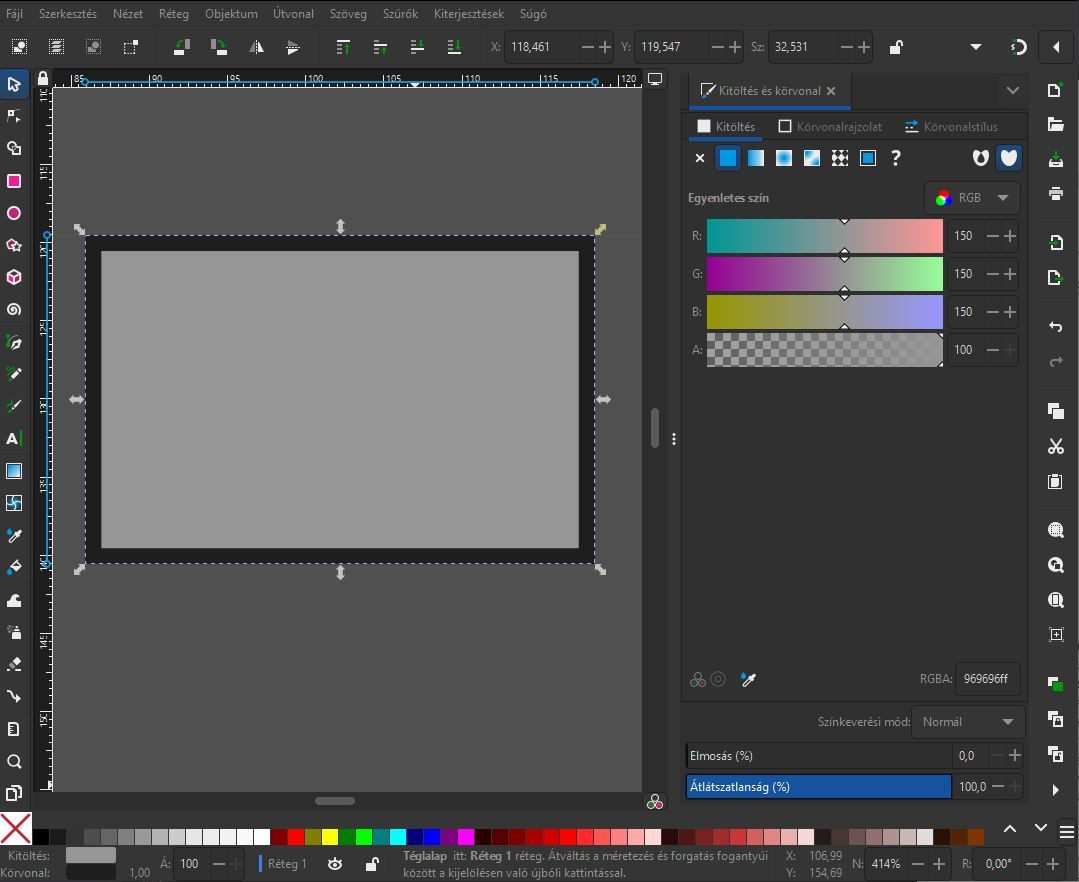
\includegraphics[width=0.8\textwidth,height=0.6\textwidth,keepaspectratio]{images/concept/inkscape.JPG}
\caption{Az Inkscape kezelőfelülete~\cite{inkscape}}
\label{fig:inkscape}
\end{figure}

Az Inkscape (\ref{fig:inkscape}. ábra) ingyenes, nyílt forráskódú asztali vektorgrafikus program Windows, macOS és Linux rendszerre~\cite{inkscape}, alapformátuma az SVG. A felülete sűrű. Bal oldalon az eszköztár, felül a menüsor és az aktuális eszköz beállításait tartalmazó sáv látható, jobb oldalon dokkolható párbeszédablakok, alul a színpaletta és az állapotsor.

Az alapalakzatok mellett csillagot, spirált és szabadkézi vonalakat is rajzol, és minden tulajdonság számszerűen is megadható a párbeszédablakokban. Az XML-szerkesztő fa szerkezetben mutatja a dokumentumot, és bármely attribútum közvetlenül módosítható benne. Az útvonalszerkesztés a program erőssége, a csomóponteszköz minden csomópontot és fogantyút elérhetővé tesz, a csomópontok típusa sarok és sima között váltható. Az útvonalakon unió, különbség, metszet, kizárás és felosztás végezhető, emellett útvonal elvágására és összevonására is van parancs~\cite{inkscape-boolean}. Az Alakzatépítő eszköz egymást metsző alakzatokból kattintásokkal állít össze új alakzatot~\cite{inkscape-1-3}.

A szöveg a vásznon és egy külön szövegablakban is szerkeszthető, útvonalra illeszthető, a betű- és sorköz és az alávágás is állítható. A színek RGB, HSL, HSV, CMYK és OKHSL színmódban adhatók meg~\cite{inkscape-1-3}. A kitöltés lehet lineáris, sugárirányú vagy hálós színátmenet és minta is. A rétegek és objektumok egy fában jelennek meg, ahol zárolhatók és elrejthetők, az illesztés pedig a rácshoz, a segédvonalakhoz és a más objektumok jellemző pontjaihoz egyaránt beállítható. Az előzmények külön panelen láthatók, az automatikus mentés pedig a beállításokban szabályozható.

\subsection{SVG-Edit}

\begin{figure}[H]
\centering
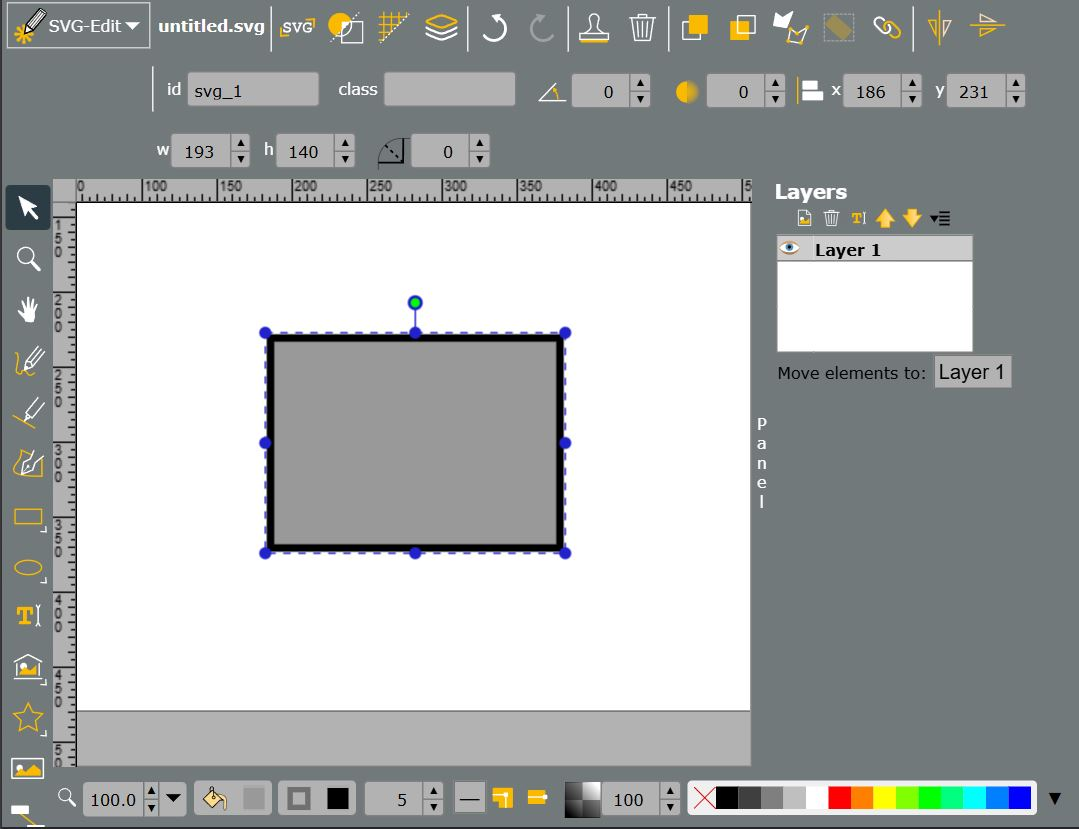
\includegraphics[width=0.8\textwidth,height=0.6\textwidth,keepaspectratio]{images/concept/svg-edit.JPG}
\caption{Az SVG-Edit kezelőfelülete~\cite{svg-edit}}
\label{fig:svg-edit}
\end{figure}

Az SVG-Edit (\ref{fig:svg-edit}. ábra) nyílt forráskódú, MIT licencű webes szerkesztő, amely regisztráció nélkül, közvetlenül a böngészőben fut~\cite{svg-edit,svgedit-github}. A felület tetején a kijelölt elem beállításai, bal oldalon az eszköztár, alul a kitöltés és a körvonal vezérlői, jobb oldalon a rétegpanel található.

Az alapalakzatok mellett egy beépített alakzatkönyvtárat is kínál. A forráskód-szerkesztő ablakban a teljes SVG-kód módosítható, a változtatások a módosítások alkalmazása után jelennek meg a vásznon. Az útvonalak csomópontjai mozgathatók, törölhetők és klónozhatók, a szakaszok típusa egyenes és görbe között váltható, a két kontrollpont pedig összekapcsolható. Logikai műveleteket nem kínál~\cite{svgedit-github}.

A szöveg a vásznon szerkeszthető, a betűstílus, a díszítővonalak, a betű- és szóköz, valamint az igazítás állítható. A beviteli mező csak egysoros szöveget fogad, és nyolc betűcsalád közül lehet választani~\cite{svgedit-github}. A színválasztó HEX, RGB és HSV értékeket fogad átlátszósággal együtt, a kitöltés egyszínű, lineáris vagy sugárirányú színátmenet lehet. Az illesztés a rácshoz kapcsolható be, az igazító parancsok több elemre is működnek. A visszavonás és a megismétlés elérhető, egy bővítmény pedig a lap bezárásakor a böngésző helyi tárolójába menti a rajzot, ha a felhasználó ezt engedélyezi.

\subsection{Boxy SVG}

\begin{figure}[H]
\centering
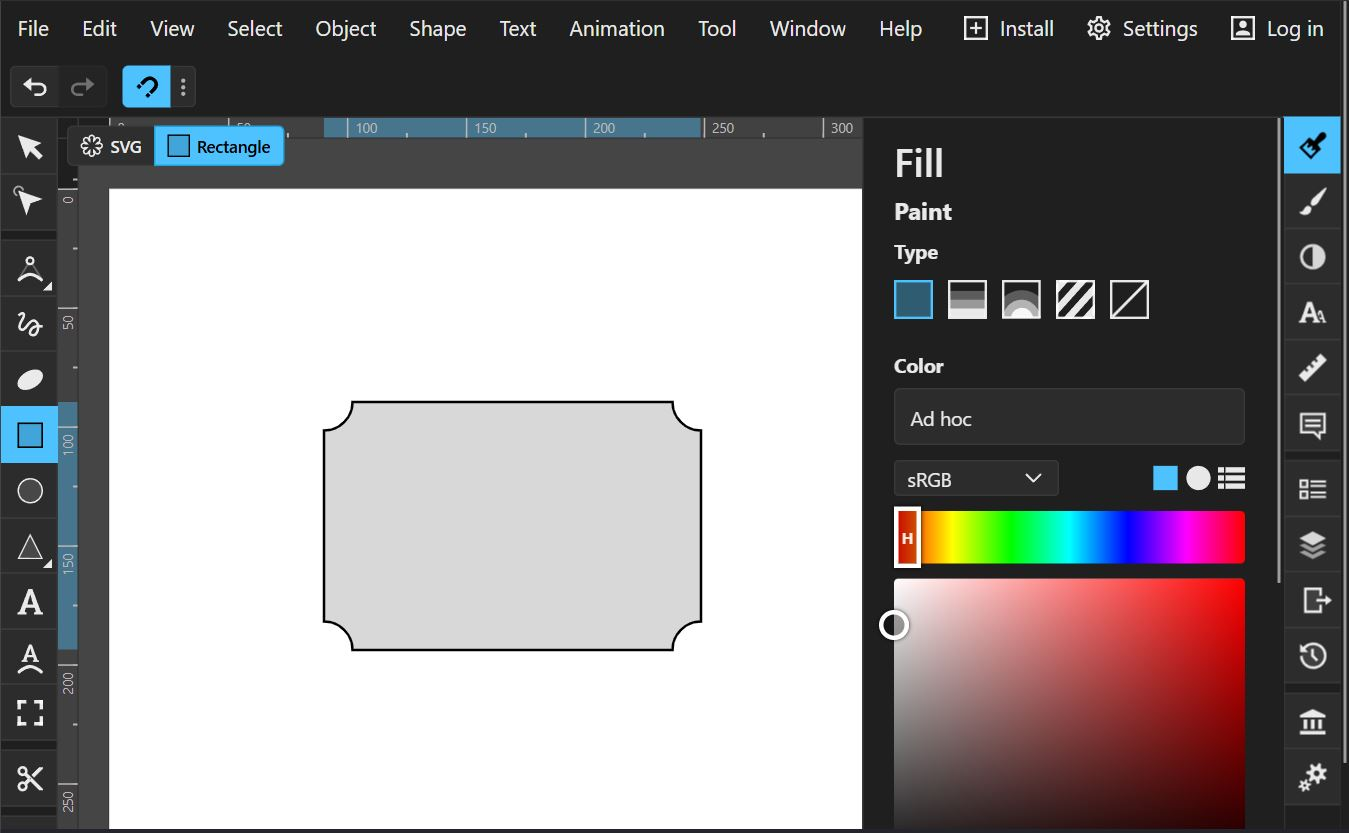
\includegraphics[width=0.8\textwidth,height=0.6\textwidth,keepaspectratio]{images/concept/boxy-svg.JPG}
\caption{A Boxy SVG kezelőfelülete~\cite{boxy-svg}}
\label{fig:boxy-svg}
\end{figure}

A Boxy SVG (\ref{fig:boxy-svg}. ábra) zárt forráskódú, freemium~\cite{freemium} vektorgrafikus szerkesztő, vagyis az alapváltozata ingyenes, a további szolgáltatásai pedig fizetősek. Webalkalmazásként és asztali alkalmazásként is elérhető. A webalkalmazás alapvető szerkesztő- és exportálási funkciói regisztráció és fizetés nélkül is használhatók, az asztali alkalmazások egy része és a haladó funkciók, például az automatikus felhőszinkronizálás és a teljes verziótörténet, viszont előfizetéshez kötöttek~\cite{boxy-svg}. A felület tetején menüsor van, alatta egy sáv a csoportosításhoz, igazításhoz, forgatáshoz és a logikai műveletekhez. A vásznat vonalzók veszik körül, a tulajdonságok a jobb oldali sávból nyíló panelekben állíthatók.

Az alapelemek mellett gyakori alakzatok, például háromszög és csillag is rajzolhatók. Az útvonalakhoz szabadkézi, másod- és harmadfokú görberajzoló eszköz tartozik, a csomópontok fogantyúkkal szerkeszthetők. Az alakzatokon unió, különbség, metszet, kizárás és felosztás végezhető. Az Elemek panel a dokumentum szerkezetét és SVG-kódját mutatja, a kód közvetlenül szerkeszthető, és az animációk kulcskockái is szerkeszthetők~\cite{boxy-svg}.

A szöveg a vásznon szerkeszthető és útvonalra illeszthető, a betűtípusok a Google Fonts gyűjteményéből, a gépre telepített vagy fájlból betöltött betűtípusok közül választhatók. A színek tizenkét színtérben adhatók meg, a szabványos és a széles színtartományú RGB-terektől az emberi színérzékelést követő CIE- és OK-modellekig, egy szöveges mezőben pedig HEX kóddal is. A kitöltés lineáris és sugárirányú színátmenet vagy minta is lehet, a gyakran használt színek, színátmenetek és minták a \lstinline[language=XML]|<defs>| elemben tárolhatók. Az elrendezést segédvonalak, intelligens segédvonalak és rács segítik, a visszavonható lépések pedig előzménypanelen láthatók.

\subsection{Figma}

\begin{figure}[H]
\centering
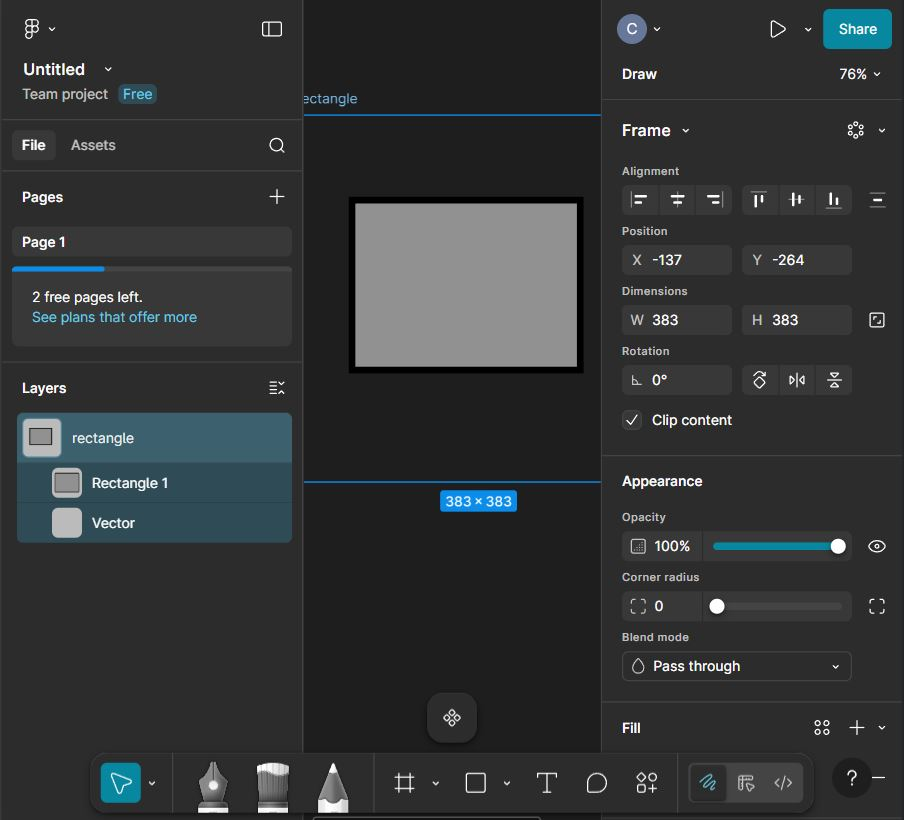
\includegraphics[width=0.8\textwidth,height=0.6\textwidth,keepaspectratio]{images/concept/figma.JPG}
\caption{A Figma kezelőfelülete~\cite{figma}}
\label{fig:figma}
\end{figure}

A Figma (\ref{fig:figma}. ábra) böngészőben és asztali alkalmazásként is futó felülettervező eszköz, amely szintén freemium konstrukcióban, ingyenes alapcsomaggal és előfizetéses csomagokkal érhető el~\cite{figma}. A rajzokat saját formátumban tárolja, az SVG számára csak importálási és exportálási formátum. A felület közepén a vászon van, bal oldalon a rétegek, jobb oldalon a tulajdonságok, az eszköztár pedig a vászon alján található~\cite{figma-ui3}.

Egy menüből téglalap, vonal, nyíl, ellipszis, sokszög, csillag és kép helyezhető el~\cite{figma-toolbar}. Az útvonalak helyett a Figma vektorhálózatokkal dolgozik, amelyekben egy csomópontból kettőnél több szakasz is indulhat~\cite{figma-vector-networks}. Az unió, a különbség, a metszet és a kizárás roncsolásmentes, az eredmény egy logikai csoport, amelynek tagjai később is módosíthatók~\cite{figma-boolean}. SVG-kódot a szerkesztő nem mutat, és az közvetlenül nem is módosítható.

A Google Fonts betűtípusai alapértelmezés szerint elérhetők, a gépre telepített betűtípusokhoz egy segédprogramra van szükség~\cite{figma-fonts}. A színválasztó HEX, HSB, HSL, CSS és RGB formátumot ismer~\cite{figma-color}, a kitöltés lehet egyszínű, színátmenet, minta, kép vagy videó. A rétegek fa szerkezetben jelennek meg. A munka folyamatosan a felhőbe mentődik, a verziótörténet az ingyenes csomagban 30 napra visszamenőleg érhető el~\cite{figma-history}.

\subsection{Mediamodifier}

\begin{figure}[H]
\centering
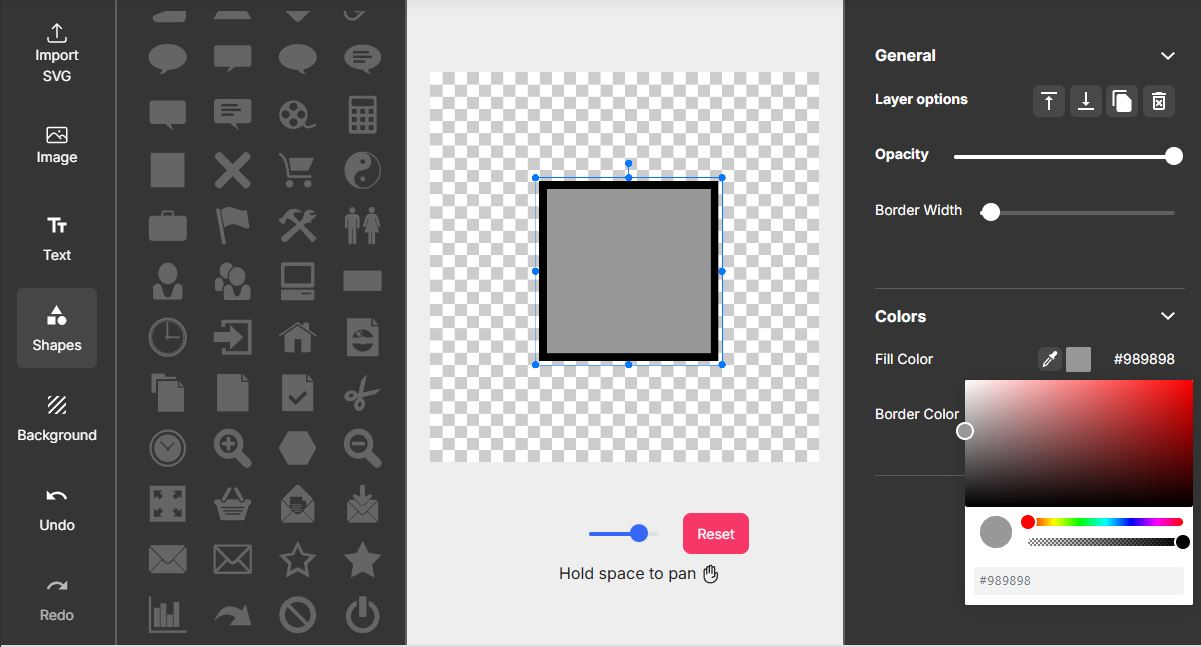
\includegraphics[width=0.8\textwidth,height=0.6\textwidth,keepaspectratio]{images/concept/mediamodifier.JPG}
\caption{A Mediamodifier kezelőfelülete~\cite{mediamodifier}}
\label{fig:mediamodifier}
\end{figure}

A Mediamodifier (\ref{fig:mediamodifier}. ábra) online grafikai és termékbemutató-készítő szolgáltatás, amely egy SVG-szerkesztőt is kínál~\cite{mediamodifier}. A szerkesztés ingyenes, a kész munka letöltéséhez azonban előfizetés szükséges. Egyszerű felületén bal oldalon az eszközsáv, jobb oldalon a tulajdonságok, középen a vászon található.

A szerkesztő kész elemek összeállítására épül. SVG-fájlok húzással helyezhetők a vászonra és kombinálhatók, az elemek csoportosíthatók, csoportbontással egyenként módosíthatók, és előrébb vagy hátrébb hozhatók~\cite{mediamodifier}. A kitöltés és a körvonal színe, valamint a körvonal vastagsága állítható. A kipróbálás során az alapalakzatok kész matricaként viselkedtek, a görbék rajzolására és az útvonalak szerkesztésére nem találtam lehetőséget, és a beimportált fájlok közül csak az egyszerű alakzatokból állók jelentek meg hibátlanul. A szöveg a vásznon szerkeszthető, de csak a betűtípus és a szín választható meg. Az SVG-kód nem érhető el.

\subsection{Összehasonlítás}
\label{sub:editor_comparison}

Az összehasonlítás szempontjait úgy választottam meg, hogy egy SVG-szerkesztő mindennapi használatát fedjék le. A felület elrendezésénél azt vizsgáltam, hogy az eszközök a megszokott helyen, logikusan csoportosítva érhetők-e el, és hogy a tulajdonságok számszerűen is megadhatók-e. Fejlesztői szempontból fontos, hogy a szerkesztő megmutatja-e az előállított SVG-kódot, és módosítható-e közvetlenül.

A rajzolás és szerkesztés szempontjai az útvonalakra összpontosítanak: hozzáadhatók és törölhetők-e a csomópontok, kényelmesen mozgathatók-e a fogantyúk, és elérhetők-e a logikai műveletek, vagyis az unió, a különbség, a metszet, a kizárás és a felosztás. Ide tartozik az illesztés a rácshoz és más objektumokhoz is. A szövegnél a többsoros bevitel, a vásznon történő szerkesztés és a betűtípusok forrása számít, a színeknél a színmegadás módjai, az átlátszóság, a színátmenetek és a minták.

A dokumentum kezelésénél a rétegek és csoportok megjelenítését, az előzményeket és a mentést vizsgáltam. A kijelölés, a nagyítás és a vágólap alapműveletei minden vizsgált szerkesztőben működtek, ezért ezeket a táblázat külön nem tünteti fel. \Aref{tab:svg-editors-comparison}. táblázat az eredményt foglalja össze.

\begin{table}[!htbp]
\caption{A vizsgált SVG-szerkesztők összehasonlítása}
\label{tab:svg-editors-comparison}
\centering
\scriptsize
\renewcommand{\arraystretch}{1.25}
\begin{adjustbox}{max width=\textwidth}
\begin{tabular}{|>{\raggedright\arraybackslash}p{2.0cm}|>{\raggedright\arraybackslash}p{2.5cm}|>{\raggedright\arraybackslash}p{2.5cm}|>{\raggedright\arraybackslash}p{2.5cm}|>{\raggedright\arraybackslash}p{2.5cm}|>{\raggedright\arraybackslash}p{2.3cm}|}
\hline
 & \textbf{Inkscape} & \textbf{SVG-Edit} & \textbf{Boxy SVG} & \textbf{Figma} & \textbf{Mediamodifier} \\ \hline
\textbf{Platform, licenc} & asztali, nyílt forráskódú & webes, nyílt forráskódú & webes és asztali, freemium & webes és asztali, freemium & webes, letöltés előfizetéssel \\ \hline
\textbf{Elrendezés} & klasszikus, dokkolható panelekkel & klasszikus, alsó stílussávval & klasszikus, beúszó panelekkel & vászon középen, eszköztár alul & egyszerű, két oldalsávval \\ \hline
\textbf{SVG-kód} & XML-szerkesztő & forrásablak, alkalmazás után frissül & Elemek panel, szerkeszthető & nincs & nincs \\ \hline
\textbf{Szöveg} & többsoros, útvonalra illeszthető & egysoros, 8 betűcsalád & útvonalra illeszthető, Google Fonts & Google Fonts, helyi betűtípusok & betűtípus és szín \\ \hline
\textbf{Színek} & RGB, HSL, HSV, CMYK, OKHSL & HEX, RGB, HSV, átlátszóság & 12 színtér (RGB, CIE, OK), HEX & HEX, HSB, HSL, CSS, RGB & színválasztó \\ \hline
\textbf{Színátmenet, minta} & lineáris, sugárirányú, hálós; minta & lineáris, sugárirányú & lineáris, sugárirányú; minta & színátmenetek, minta, kép & egyszínű \\ \hline
\textbf{Útvonalak} & teljes csomópont-szerkesztés & csomópontok, szakasztípus & csomópontok, fogantyúk & vektorhálózatok & nincs \\ \hline
\textbf{Logikai műveletek} & unió, különbség, metszet, kizárás, felosztás & nincs & unió, különbség, metszet, kizárás, felosztás & unió, különbség, metszet, kizárás & nincs \\ \hline
\textbf{Illesztés} & rács, segédvonalak, objektumok & rács & rács, segédvonalak & igazítási segédvonalak & alapszintű \\ \hline
\textbf{Rétegek} & objektumfa, zárolás & rétegpanel & elemfa & rétegfa & előre-hátra mozgatás \\ \hline
\textbf{Előzmények, mentés} & előzménypanel, automatikus mentés & visszavonás, mentés a lap bezárásakor & előzménypanel, felhőtárhely & verziótörténet, folyamatos felhőmentés & letöltés előfizetéssel \\ \hline
\end{tabular}
\end{adjustbox}
\end{table}

\subsection{Következtetések és célkitűzések}
\label{sub:editor_conclusions}

A vizsgált szerkesztők közül az Inkscape kínálja a legteljesebb SVG-szerkesztést, de asztali program, amelyet telepíteni kell. A Boxy SVG hasonlóan sokoldalú, böngészőben is fut, haladó funkciói azonban előfizetéshez kötöttek, és a forráskódja zárt. A Figma kiváló vektoros eszközei saját adatmodellre épülnek, az SVG csak be- és kimeneti formátum. A Mediamodifier kész elemek összeállítására készült, görbéket nem lehet vele rajzolni. Az SVG-Edit ingyenes és nyílt forráskódú, kódnézetet is kínál, de csak egysoros szöveget kezel, és logikai műveletek nincsenek benne.

% A vizsgált alkalmazások többsége a klasszikus elrendezést követi, amely más grafikai programokból is ismerős.

Ezek alapján a saját szerkesztővel szemben a következő célokat tűztem ki:

\begin{enumerate}
\item A szerkesztő szerver, telepítés és regisztráció nélkül, ingyenesen fusson a böngészőben, klasszikus elrendezéssel.
\item Kínáljon a vizsgált szerkesztőkhöz mérhető rajzoló és szerkesztő eszközöket, köztük teljes értékű útvonalszerkesztést és logikai műveleteket, amelyek eredménye görbékből álló, tovább szerkeszthető alakzat marad.
\item Kezeljen többsoros szöveget, és alakítsa útvonallá úgy, hogy az eredmény megegyezzen a képernyőn látottal.
\item Importáljon SVG-fájlokat, és jelezze, milyen szerkezeteket nem tud kezelni.
\item Exportáljon szabványos SVG-fájlt és raszteres képet.
\item Legyen telefonon és táblagépen is kezelhető.
\end{enumerate}

\Aref{ch:requirements}. fejezet ezeket a célokat bontja részletes követelményekre, \aref{ch:evaluation}. fejezet pedig azt értékeli, mennyiben teljesültek.
